\documentclass{article}

 % \usepackage[utf8]{inputenc} %Stationær ÆØÅ
\usepackage[ansinew]{inputenc} %Bærbar ÆØÅ?

%\usepackage{url} % Allows hyperlinks
\usepackage[hyphens]{url} %URLs
\usepackage{graphicx} % Allows figures
% \usepackage{etoolbox} %for configuration of sloppy

%Section style
\usepackage{xcolor}

\definecolor{secnum}{RGB}{102,102,102} 

\makeatletter
    \def\@seccntformat#1{\llap{\color{secnum}\csname the#1\endcsname\hskip 16pt}}
\makeatother
%end section style

% \apptocmd{\sloppy}{\hbadness 10000\relax}{}{} %adds hbadness to sloppy
\setlength{\paperheight}{297mm} %Sets the page to an A4
\setlength{\paperwidth}{210mm}	%Sets the page to an A4

\begin{document}

\begin{titlepage}
\begin{center}
\textsc{\Large IT Sikkerhed}\\[0.5cm]
\textsc{OPGAVE B: Sikkerhedsanalyse af sociale medier}\\[0.5cm]
\vspace{2 cm}
\begin{tabular}{ll}
Kasper Passov & pvx884\\
\end{tabular}
\end{center}
\vspace{5 cm}
\newpage
\tableofcontents
\end{titlepage}

\section{Resumé af firma og system}
\subsection{Firmaets risiko niveau}
Firmaet BIOmedix er et firma med høj sårbarhed overfor informations tyveri. En lækage af forsknings resultater kan have meget alvorlige konseknverser for BIOmedix, da salg af disse resultater og patenter der er kommet deraf er deres primære inkomstkilde. Dette betyder IT sikkerheden bør være i firmaets fokus for at beskytte disse aktiver. 

\subsection{Resumé af det nye system}
Der skal indføres fire nye sociale medier i BIOmedix. Dette har jeg valgt at dele op i 2 grupper. 

\paragraph{Eksterne systemer}
Den ene er 3 sider i de sociale netværker Facebook, Twitter og LinkedIn som jeg vil kalde de eksterne systemer, idet pointer med disse er at give firmaet en mulighed for at kommunikere med folk udenfor firmaet. Jeg har valgt at samle disse systemer i en gruppe da jeg mener der er mange ligheder i hvilke trusler og sårbarheder disse systemer bliver udsat for, og derigennem skal sikkerheden i disse systemer håndteres ens. Kodeord og brugernavne til disse kontoer bliver holdt af kommunikationsafdelingen, som står for opdateringer.

\paragraph{Internt system}
Det sidste system, Yammer, er et lukket socialt netværk for alle firmaets ansatte. Systemet lader dem blandt andet opdatere arbejdsstatus og danne projektgrupper. Jeg vil referer til dette netværk som et internt system, da mange af de trusler og sårbarheder Yammer er udsat for ville kunne bruges på lignende systemer i fremtiden.

\subsection{Sikkerhedsmål}

Sikkerheds målet for de tre eksterne netværker, er at have beskyttede kontier og passwords,
samt at have siderne let tilgængelige. Det interne system Yammer, skal have adgangsniveauer
så hver ansat kun har tilgang til det nødvendige. Ud over at beskytte kontierne skal de ansatte
have nem adgang til siden.

\section{Aktiver}
\subsection{Eksterne systemer}
Vores vigtigste aktiv i de eksterne systemer er muligheden for at videregive information til den bredere befolkning. 

\subsection{Interne systemer}
Informationen på det interne system Yammer skal beskyttes fra udekommende, da der vil være store mængder af kritisk information på dette netværk. Derudover skal ansatte have nem og hurtig adgang til information, gerne hvor som helst og når som helst.

\subsection{Begrundelse for aktiver}

\paragraph{Spredning af information}
De eksterne systemers primære funktion er at give firmaet en kommunikations kanal til den brede befolkning. Dette kan både være en nyhed om et gennembrud, et opslag til en ny stilling eller general information om firmaet. Denne aktiv skal beskyttes ved at holde kommunikations linjen åben og så uhindret som mulig.

\paragraph{Information på det interne system}
Yammer kommer til at indeholde hvad de ansatte arbejder på, hvem de arbejder med, forskningsidéer og filer. Et brud på dette netværk vil blotte alt information BIOmedix har, og gøre det muligt for konkurrenter eller patenttrolde at se hvor langt BIOmedix er med et stykke forskning, og muligvis presse en patent frem inden BIOmedix kan færdiggøre sig. 

\paragraph{Adgang til Yammer}
Uden de ansattes adgang til Yammer, vil dette cloud system ikke være sikkerheds risikoen værd. Derfor skal det gøres så nemt som muligt for de ansatte at få adgang til Yammer, gerne både på arbejdspladsen og i hvert ansats hjem.  


\section{Trusselsaktører}

\paragraph{Hackere}

\paragraph{Konkurenter}

\paragraph{Ultilfredse ansatte}

\section{Trusler}

\subsection{komprimering af udbyders side}

\subsection{Ansatte's passwords komprimenteres}

\subsection{Utilfredse ansatte lækker fortrolig information}

\subsection{Relevante angreb}

\subsubsection{AP's Twitter-konto}

\begin{figure}
  \begin{center}
    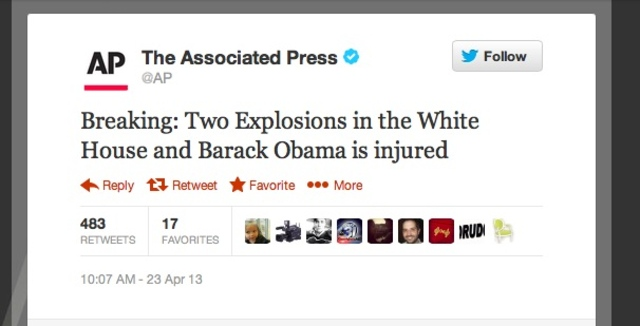
\includegraphics[width=0.6\textwidth]{../Pictures/APTweet.jpg}
  \end{center}
  \caption{Tweeten fra hackeren over nyhedsbureauet Associated Press \cite{APTweetSource}}
  \label{fig:Tweet}
\end{figure}

\paragraph{Angreb}

To af Associated Press' twitter sider blev den 23 april 2013 hacket of en falsk nyhedsmeddelse blev udsendt. Tweetet kan ses på figur \ref{fig:Tweet}

\paragraph{Relevans for BIOmedix}

Et sådan angreb på BIOmedix kan fjerne tilhængernes tiliden til de externe sider, da følgere til siderne
ønsker nyheder fra BIOmedxi og ikke missinformation. Derudover kan en sådan hacking lade konkurrenter
samt ondsindede hacker sprede misinformation i BIOmedix navn. 

\subsubsection{LinkedIn password-lækage}

\paragraph{Angreb}
På et forum lagde brugeren "dwdm" 8 millioner crypterede passwords op og bad om hjælp
til at bryde dem. Det viser sig at de 8 millioner passwords blandt andet er fra siden LinkedIn.
Det spekuleres at angriberen allerede havde brudt de en meget stor del af LinkedIn's brugere, da
der var omkring 120 millioner brugere på LinkedIn's side da listen blev frigjort. Dette kan betyde
at "dwdm" allerede havde brudt de svagere passwords, og de 8 millioner var det subset af passwords
han ikke kunne bryde alene\cite{LinkedInStory}.

\paragraph{Relevans for BIOmedix}

Et stort lækage af passwords fra en sådan side kunne betyde alle BIOmedix'
sociale medie sider ville være usikre, hvis det samme password og brugernavn var 
brugt overalt.
Hvis en sådan lækage skete og blev kendt, skal passworded på den pågældene side, samt
alle sider der benytter det samme password ændres. Derefter skal alt information på
siden tjekkes igennem for ændringer.
Selvom et sådan angreb næppe er gjort af nogen der er intereseret i BIOmedix siden, er
det muligt listen af passwords er blevet solgt til en intereseret konkurent. Derfor kan
det ikke ignoreres selv hvis det ikke er konkurenter der har lavet angrebet.

\subsubsection{Ex-CIA ansat påstår at have vidergivet NSA hemmeligheder} 

\paragraph{Angreb}
En tidligere CIA agent påstår at være kilden til de hemmelige dokumenter der er blevet
lækket til flere nyhedssider. Den lækkede information omhandler et program kaldet PRISM 
den amerikanse efterretningstjeneste bruger til at spionere på privat personer.

\paragraph{Relevans for BIOmedix}
En utilfreds ansat ville kunne videregive fortrogelig information. Et eksempel kunne være hvilken
forskning BIOmedix er igang med. Denne information kunne være interesant for konkurenter, da det ville
give dem muligheden for at forske i det samme, og potentielt tage en patent eller udgive resultater
inden BIOmedix er klar til det.


\section{Sårbarheder}

Ansattes password styrke.
Kritisk information er ikke på firmastyret servere.
Fishing attempts
En bruger på alle tre sider
Social netværk hacket

\section{Modforanstaltninger}

\section{Risici}

\section{Foreslåede modforanstaltninger}

\paragraph{Firewall for Yammer}
Så kun ip'er fra biomedix kan logge på

\paragraph{Password kursus til medarbejdere}

Password styrke og brug

\section{Konklusion}


\newpage
\begin{thebibliography}{100}


\bibitem{APTweetSource}
\url{www.businessinsider.com/ap-hacked-obama-injured-white-house-explosions-2013-4}
\bibitem{APTweetStory} 
\url{www.guardian.co.uk/business/2013/apr/23/ap-tweet-hack-wall-street-freefall}
\bibitem{LinkedInStory}
\url{http://arstechnica.com/security/2012/06/8-million-leaked-passwords-connected-to-linkedin}
\end{thebibliography}
\end{document}
